% =============================================================
% Capítulo 4. Propuesta
% =============================================================
% Descripción conceptual del sistema (el algoritmo genético):
% ciclo, representación, fitness, cruce, mutación, torneo, evaluación
% y, al final, el pipeline que lo integra. SIN nombres de código.
% Los experimentos que validan estas decisiones están en el cap. Desarrollo.
% =============================================================

\chapter{Propuesta}
\label{sec:arquitectura}

La metodología iterativa descrita en el capítulo anterior condujo, decisión a decisión, al sistema que aquí se presenta. Este capítulo describe la propuesta: un algoritmo genético adaptado a la construcción de mazos cuya función de fitness se evalúa mediante la simulación de partidas. La exposición sigue un orden conceptual. En primer lugar se presenta el ciclo evolutivo a nivel general. A continuación se detallan sus componentes: la representación de un mazo como individuo, la función de fitness que mide su calidad, y los operadores de cruce, mutación y selección que gobiernan la evolución. Después se describe la evaluación por simulación, que proporciona la medida de rendimiento. Por último, se expone el flujo completo (\emph{pipeline}) que integra todas las etapas en un sistema ejecutable.

\section{El ciclo evolutivo}
\label{sec:ciclo}

El núcleo de la propuesta es un algoritmo genético que mantiene una población de mazos y la hace evolucionar a lo largo de un número fijo de generaciones. La figura~\ref{fig:bucle} resume el ciclo que se repite en cada generación.

\begin{figure}[H]
\centering
\begin{tikzpicture}[
    font=\small,
    paso/.style={draw, rounded corners, align=center, minimum height=0.95cm, text width=2.0cm, fill=blue!5},
    flecha/.style={-{Stealth[length=2.4mm]}, thick}
]
\node[paso] (pop) {Población gen.\,$g$};
\node[paso, right=0.85cm of pop] (eval) {Evaluación\\(Swiss + Forge)};
\node[paso, right=0.85cm of eval] (sel) {Selección\\por torneo};
\node[paso, right=0.85cm of sel] (cruce) {Cruce y\\mutación};
\node[paso, right=0.85cm of cruce] (nueva) {Población gen.\,$g{+}1$};
\node[paso, fill=orange!10, below=1.0cm of eval] (hof) {Hall of Fame\\(élite)};
\draw[flecha] (pop) -- (eval);
\draw[flecha] (eval) -- (sel);
\draw[flecha] (sel) -- (cruce);
\draw[flecha] (cruce) -- (nueva);
\draw[flecha] (eval) -- (hof);
\draw[flecha] (hof.south) -- ++(0,-0.35) -| (nueva.south) node[pos=0.25, below, font=\scriptsize] {elitismo};
\draw[flecha] (nueva.north) -- ++(0,0.55) -| (pop.north) node[pos=0.25, above, font=\scriptsize] {nueva generación};
\end{tikzpicture}
\caption{Ciclo generacional del algoritmo. La evaluación alimenta el Hall of Fame, que inyecta la élite en la población siguiente mediante elitismo.}
\label{fig:bucle}
\vspace{2pt}
{\footnotesize Fuente: elaboración propia.}
\end{figure}

La población inicial no es completamente aleatoria. A cada mazo de partida se le asigna un arquetipo objetivo (aggro, midrange o control) con cuotas iguales, y su estructura se consolida hacia ese arquetipo. Esta asignación es solo una siembra: en cuanto comienza la evolución, el arquetipo de cada mazo se redetecta de forma dinámica y puede cambiar si la presión selectiva lo recompensa. Con ello se garantiza diversidad de arquetipos desde la primera generación sin fijarla de manera artificial.

A partir de ahí, cada generación sigue el mismo ciclo. Primero se preserva la élite: los mejores mazos históricos, almacenados en una estructura denominada Hall of Fame, pasan intactos a la nueva población. El resto se genera por reproducción. Cada par de progenitores se elige por selección de torneo, se combina mediante el operador de cruce con una cierta probabilidad y se altera mediante el operador de mutación con otra probabilidad. La nueva población se evalúa, se actualizan el Hall of Fame y las estadísticas de la ejecución, y se conserva una copia de seguridad del estado. El ciclo se repite hasta agotar el número de generaciones previsto o alcanzar un valor de fitness objetivo.

La intensidad de la mutación no es constante. Se incrementa cuando el algoritmo detecta un estancamiento, es decir, varias generaciones sucesivas sin mejorar el mejor fitness, y se relaja en la fase final si la población converge sin atascarse. El ajuste es aditivo y se mantiene dentro del intervalo $[0.1,\ 1.0]$, de modo que cada episodio de estancamiento aporta un incremento perceptible en lugar de saturar la tasa de forma abrupta.

El Hall of Fame conserva los mejores mazos históricos con una cuota estricta por arquetipo: reserva un tercio de sus plazas a cada uno de los tres arquetipos, y si un arquetipo carece de candidatos suficientes, sus plazas quedan vacías en lugar de cederse a otro. Esta restricción preserva la diversidad, ya que impide que el arquetipo dominante en un momento dado monopolice la élite y arrastre a toda la población hacia una única estrategia.

\section{Representación del individuo}
\label{sec:representacion}

Cada individuo de la población es un mazo, y se representa como un vector de enteros cuya longitud coincide con el número de cartas del catálogo. La posición $i$ del vector indica cuántas copias de la carta de identificador $i$ contiene el mazo. Un mazo de sesenta cartas es, por tanto, un vector disperso (la mayoría de sus componentes son cero) cuyos valores suman sesenta. La figura~\ref{fig:individuo} ilustra esta representación.

\begin{figure}[H]
\centering
\begin{tikzpicture}[font=\small,
    celda/.style={draw, minimum width=0.9cm, minimum height=0.75cm}]
\node[celda] (c0) {0};
\node[celda, right=0pt of c0] (c1) {0};
\node[celda, right=0pt of c1, fill=blue!10] (c2) {4};
\node[celda, right=0pt of c2] (c3) {0};
\node[celda, right=0pt of c3, fill=red!10] (c4) {1};
\node[celda, right=0pt of c4] (c5) {$\cdots$};
\node[celda, right=0pt of c5, fill=blue!10] (c6) {4};
\node[celda, right=0pt of c6] (c7) {$\cdots$};
\node[celda, right=0pt of c7, fill=green!12] (c8) {24};
\node[below=1pt of c0, font=\scriptsize, text=gray] {0};
\node[below=1pt of c1, font=\scriptsize, text=gray] {1};
\node[below=1pt of c2, font=\scriptsize, text=gray] {2};
\node[below=1pt of c4, font=\scriptsize, text=gray] {4};
\node[below=1pt of c6, font=\scriptsize, text=gray] {$i$};
\node[below=1pt of c8, font=\scriptsize, text=gray] {$N\!-\!1$};
\node[above=1pt of c2, font=\scriptsize, align=center, text=blue!50!black] {pack de\\4 copias};
\node[above=1pt of c4, font=\scriptsize, align=center, text=red!60!black] {1 copia};
\node[above=1pt of c8, font=\scriptsize, align=center, text=green!45!black] {tierra\\básica};
\end{tikzpicture}
\caption{Representación de un mazo como vector de enteros. Cada posición corresponde a una carta del catálogo y su valor indica el número de copias en el mazo; la suma de todas las componentes es sesenta.}
\label{fig:individuo}
\vspace{2pt}
{\footnotesize Fuente: elaboración propia.}
\end{figure}

Esta representación aporta dos ventajas. Por una parte, permite operar sobre los mazos con álgebra vectorial, lo que agiliza el cruce y el cálculo de la diversidad de la población. Por otra, traduce de forma directa la norma de las cuatro copias: el valor de cada componente está acotado a cuatro para las cartas no básicas, y únicamente las tierras básicas pueden superar ese límite. El vector constituye el genotipo del individuo; el fenotipo es el mazo reconstruido a partir de él, con sus cartas y sus atributos, que es lo que el simulador necesita para jugar.

\section{Función de fitness}
\label{sec:fitness}

La función de fitness asigna a cada mazo un valor numérico que mide su calidad como solución y orienta toda la evolución. Combina dos criterios mediante una suma ponderada:

\begin{equation}
\text{fitness} = \alpha \cdot \text{tasa\_de\_victorias} + \beta \cdot \text{calidad},
\qquad \alpha = 0.7,\quad \beta = 0.3.
\label{eq:fitness}
\end{equation}

El primer criterio de la ecuación~\ref{eq:fitness}, la tasa de victorias, mide el rendimiento real del mazo: la proporción de partidas que gana en el torneo frente a otros mazos de la población, según se describe en la sección~\ref{sec:torneo}. El segundo criterio, la calidad, valora cómo de bien construido está el mazo desde un punto de vista estructural, con independencia de su resultado en las partidas.

Los coeficientes $\alpha$ y $\beta$ ponderan la importancia relativa de cada criterio y suman la unidad. La tasa de victorias recibe el peso mayor porque mide directamente el objetivo del sistema, que es ganar partidas, mientras que la calidad estructural actúa como criterio secundario y como regularizador. Su función es doble. Por un lado desempata entre mazos con un rendimiento similar en favor del que está mejor construido. Por otro evita que el algoritmo premie mazos que ganan por circunstancias del entorno de evaluación pero carecen de coherencia interna. Los valores concretos, $\alpha = 0.7$ y $\beta = 0.3$, no se fijaron de forma arbitraria. Parten de una configuración inicial de $0.6$ y $0.4$ que se reajustó al comprobar que la métrica de calidad había perdido capacidad de discriminación (sección~\ref{sec:refinamiento}), lo que aconsejaba rebajar su peso sin llegar a anularlo. Una calibración más fina de estos coeficientes, mediante un análisis de sensibilidad que barra distintas proporciones, se plantea como línea de trabajo futuro.

La calidad se evalúa en el intervalo $[0, 1]$ sobre el arquetipo que el mazo exhibe en cada momento, detectado a partir de su coste de maná medio y de su número de criaturas. Agrega tres componentes estructurales, cada uno normalizado en $[0, 1]$, mediante una media ponderada:

\begin{equation}
\text{calidad} = 0.35\cdot\text{sinergia} + 0.35\cdot\text{equilibrio} + 0.30\cdot\text{coherencia}.
\label{eq:calidad}
\end{equation}

Cada componente de la ecuación~\ref{eq:calidad} mide una propiedad distinta de la construcción:

\begin{itemize}
    \item La \textbf{sinergia} valora la cohesión interna del mazo a partir de tres factores: la concentración en un mismo tipo de criatura (sinergia tribal), la densidad de habilidades clave (como el vuelo o el arrollar) y la consistencia cromática, que penaliza el uso de un número excesivo de colores.
    \item El \textbf{equilibrio de categorías} compara las proporciones de tierras, criaturas y hechizos del mazo con los rangos ideales del arquetipo detectado.
    \item La \textbf{coherencia de arquetipo} contrasta el coste de maná medio, el número de criaturas y el número de tierras del mazo con los valores característicos de ese arquetipo.
\end{itemize}

Los pesos de esta ponderación no son uniformes por casualidad. Reflejan la capacidad de discriminación de cada componente, medida por su coeficiente de variación sobre la población, de modo que la sinergia y el equilibrio de categorías, que discriminan más entre mazos, pesan más que la coherencia de arquetipo. Esta ponderación es, además, el resultado de un refinamiento. Una versión inicial de la métrica incorporaba tres componentes adicionales (la estructura de \emph{playsets} de cuatro copias, el poder bruto de las cartas estimado a partir de su rareza y eficiencia, y el ajuste de la curva de maná al ideal del arquetipo), que se retiraron al comprobar que, tras la mejora estructural de los mazos, habían dejado de discriminar entre unos y otros. Ese análisis y la recalibración resultante se detallan en la sección~\ref{sec:refinamiento}.

La función admite, además, un tercer criterio opcional: el rendimiento frente a un conjunto de mazos de referencia del metajuego real, denominado \emph{gauntlet}. Este componente se exploró y finalmente se descartó por los motivos que se exponen en la sección~\ref{sec:gauntlet}.

\section{Operador de cruce}
\label{sec:cruce}

El cruce combina el material de dos progenitores para formar descendientes y dispone de dos variantes que se eligen al azar en cada reproducción. El cruce uniforme decide carta por carta de cuál de los dos progenitores hereda cada posición del descendiente. El cruce por categoría decide por bloques. Cada descendiente hereda la base de tierras completa de uno de los progenitores, las criaturas completas del otro y los hechizos del que corresponda, mientras que su hermano recibe la herencia complementaria. De este modo se preserva la coherencia interna de cada bloque en lugar de fragmentarlo por un punto de corte arbitrario. La figura~\ref{fig:cruce} ilustra esta segunda variante y los dos descendientes que produce.

\begin{figure}[H]
\centering
\begin{tikzpicture}[
    font=\small,
    mazo/.style={draw, rounded corners, align=left, text width=2.9cm, fill=gray!5, inner sep=5pt},
    flecha/.style={-{Stealth[length=2.4mm]}, thick}
]
\node[mazo, fill=blue!4] (A) {\textbf{Progenitor A}\\[2pt] Tierras\\ Criaturas\\ Hechizos};
\node[mazo, fill=orange!6, below=0.9cm of A] (B) {\textbf{Progenitor B}\\[2pt] Tierras\\ Criaturas\\ Hechizos};
\node[circle, draw, fill=gray!15, inner sep=1.6pt, right=1.5cm of A, yshift=-0.85cm] (j) {};
\node[mazo, right=1.5cm of j, yshift=1.4cm] (D1) {\textbf{Descendiente 1}\\[2pt] \textcolor{blue!65!black}{Tierras (A)}\\ \textcolor{orange!80!black}{Criaturas (B)}\\ \textcolor{blue!65!black}{Hechizos (A)}};
\node[mazo, right=1.5cm of j, yshift=-1.4cm] (D2) {\textbf{Descendiente 2}\\[2pt] \textcolor{orange!80!black}{Tierras (B)}\\ \textcolor{blue!65!black}{Criaturas (A)}\\ \textcolor{orange!80!black}{Hechizos (B)}};
\draw[flecha, blue!65!black] (A.east) -- (j);
\draw[flecha, orange!80!black] (B.east) -- (j);
\draw[flecha] (j) -- (D1.west);
\draw[flecha] (j) -- (D2.west);
\end{tikzpicture}
\caption{Cruce por categoría. Cada bloque de cartas (tierras, criaturas o hechizos) se hereda íntegro de uno de los dos progenitores, lo que preserva su coherencia interna. La operación produce dos descendientes complementarios. El descendiente 1 hereda las tierras y los hechizos del progenitor A y las criaturas del B, y el descendiente 2 recibe la herencia inversa.}
\label{fig:cruce}
\vspace{2pt}
{\footnotesize Fuente: elaboración propia.}
\end{figure}

\section{Operador de mutación pack-aware}
\label{sec:mutacion}

La mutación introduce variaciones en un mazo y constituye uno de los elementos diferenciales de la propuesta, ya que opera sobre conjuntos de cuatro copias (\emph{packs}) y no sobre copias sueltas. Todas sus variantes comparten un principio: cada mutación es una sustitución atómica que retira un pack y añade otro, manteniendo constante el número de cartas, tal como ilustra la figura~\ref{fig:mutacion}.

\begin{figure}[H]
\centering
\begin{tikzpicture}[
    font=\small,
    mazo/.style={draw, rounded corners, align=left, text width=3.1cm, fill=gray!5, inner sep=6pt},
    flecha/.style={-{Stealth[length=2.8mm]}, very thick}
]
\node[mazo] (antes) {\textbf{Mazo (60 cartas)}\\[2pt] 24 Tierras\\ 4$\times$ Carta C\\ \textcolor{red!75!black}{4$\times$ Carta A}\\ 4$\times$ Carta D\\ \dots};
\node[mazo, right=3.4cm of antes] (despues) {\textbf{Mazo (60 cartas)}\\[2pt] 24 Tierras\\ 4$\times$ Carta C\\ \textcolor{green!45!black}{4$\times$ Carta B}\\ 4$\times$ Carta D\\ \dots};
\draw[flecha] (antes) -- node[above, align=center, font=\scriptsize] {intercambio\\de pack} node[below, align=center, font=\scriptsize] {$-$ pack baja afinidad\\$+$ pack alta afinidad} (despues);
\end{tikzpicture}
\caption{Mutación a nivel de pack. La operación retira las cuatro copias de una carta poco afín al arquetipo e introduce cuatro de otra más afín, conservando el total de sesenta cartas.}
\label{fig:mutacion}
\vspace{2pt}
{\footnotesize Fuente: elaboración propia.}
\end{figure}

La propuesta define siete operadores de mutación. El operador genérico intercambia una carta de baja afinidad con el arquetipo por otra de alta afinidad. Los seis restantes modelan decisiones concretas de un jugador que construye un mazo: completar un pack parcial hasta las cuatro copias, aproximar la curva de maná al ideal del arquetipo, incorporar cartas de respuesta cuando faltan, podar un color secundario para consolidar la base de tierras, sustituir una criatura por otra de igual coste y mejores características, y reforzar la tribu dominante (el tipo de criatura predominante, que habilita sinergias tribales). Cuando un operador temático no encuentra candidatos viables, recurre al intercambio genérico, de modo que ninguna mutación queda sin efecto. Un mecanismo de reparto pondera los siete operadores según el régimen evolutivo: durante el estancamiento prima el intercambio exploratorio, mientras que en marcha normal el peso se distribuye entre la consolidación y los operadores temáticos.

Tras cualquier operación de cruce o mutación, una función de reparación restablece el cumplimiento de las restricciones del formato. Consolida los \emph{singletons} sobrantes (cartas presentes en una sola copia) hasta dejar un máximo de dos, ajusta el total a sesenta cartas, impone el número mínimo de tierras propio del arquetipo (veinte para aggro, veintitrés para midrange y veinticinco para control), garantiza al menos una tierra básica por cada color empleado y rebalancea la base de tierras para que las fuentes de cada color sean proporcionales a su demanda, según la heurística de Karsten descrita en la ecuación~\ref{eq:karsten}. Esta reparación es la garante de las restricciones duras del formato.

\section{Selección y sistema de torneo}
\label{sec:torneo}

La selección de progenitores se realiza por torneo: se toma una muestra aleatoria de la población y se elige el individuo de mayor fitness, lo que regula la presión selectiva mediante el tamaño de la muestra. La evaluación del fitness, en cambio, exige enfrentar los mazos entre sí, y la forma de emparejarlos dentro de una generación determina cuántas partidas hay que simular, número que domina el coste de todo el sistema.

El diseño admite dos esquemas de emparejamiento. El round-robin completo enfrenta cada mazo contra todos los demás: para una población de $N$ mazos genera $\binom{N}{2}$ enfrentamientos, un coste que crece con el cuadrado del tamaño. El Swiss Tournament, en cambio, hace que cada mazo dispute un número fijo de rondas $k$ contra rivales distintos, lo que genera del orden de $N \cdot k / 2$ enfrentamientos, un coste que crece de forma aproximadamente lineal. La figura~\ref{fig:swiss} compara ambos esquemas.

\begin{figure}[H]
\centering
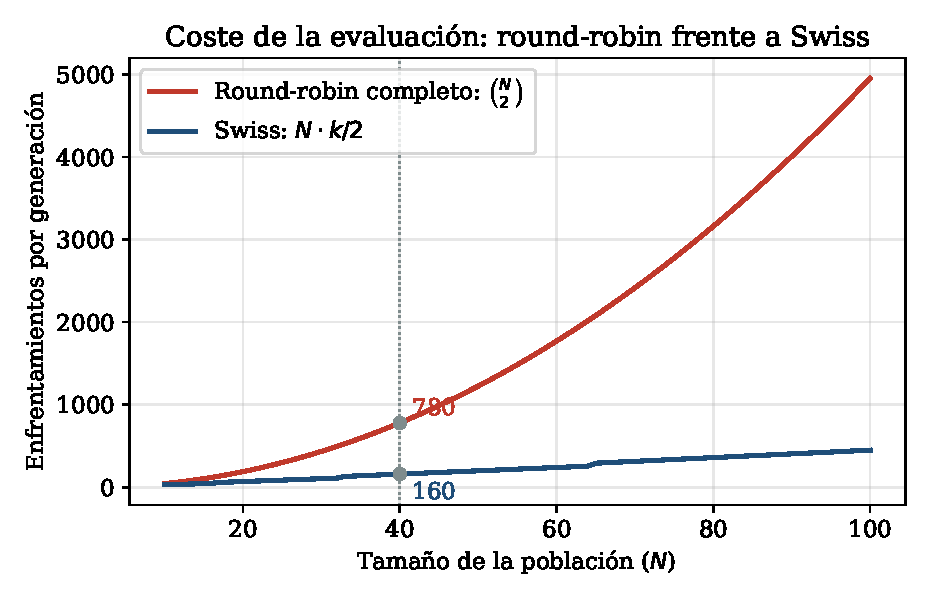
\includegraphics[width=0.78\textwidth]{images/fig_swiss_vs_roundrobin.pdf}
\caption{Número de enfrentamientos por generación según el tamaño de la población. El punto de trabajo del sistema ($N=40$) pasa de 780 enfrentamientos en round-robin a 160 en Swiss.}
\label{fig:swiss}
\vspace{2pt}
{\footnotesize Fuente: elaboración propia.}
\end{figure}

La diferencia tiene consecuencias prácticas. Para una población de cuarenta mazos, el round-robin completo exige 780 enfrentamientos por generación, mientras que el Swiss con ocho rondas exige 160, una reducción cercana al 80\,\%. El Swiss presenta una segunda ventaja: es el sistema con el que se disputan los torneos reales de Magic, de modo que su adopción aproxima la evaluación a las condiciones de competición que el trabajo pretende reproducir. El paso del round-robin al Swiss constituye uno de los ejes de la evolución del sistema, que se detalla en la sección~\ref{sec:evolucion}.

\section{Evaluación por simulación con Forge}
\label{sec:evaluacion}

La tasa de victorias que alimenta la función de fitness no se estima con una heurística, sino que se mide jugando. Cada enfrentamiento se resuelve en el simulador Forge, que disputa tres partidas entre dos mazos con jugador inicial aleatorio en cada una; el sistema interpreta el resultado, cuenta las victorias y determina el ganador. Esta integración convierte la evaluación en una medida de rendimiento real bajo el reglamento completo del juego, y no en una aproximación.

El coste de simular partidas reales obliga a paralelizar la evaluación. Los enfrentamientos de una misma generación se reparten entre varios procesos, cuyo número se fija en función de los núcleos de cómputo disponibles. Un límite de tiempo adaptativo evita que una partida bloqueada detenga la ejecución: si se acumulan interrupciones por tiempo, el límite se eleva de forma automática. En las ejecuciones reales, la tasa de partidas fallidas se mantiene por debajo del 0.1\,\%, lo que confirma que la integración con el simulador es estable a lo largo de decenas de horas de cómputo.

\section{Integración: el pipeline del sistema}
\label{sec:pipeline}

Los componentes descritos se integran en un flujo de tres etapas encadenadas, coordinadas por un módulo orquestador, que la figura~\ref{fig:pipeline} resume.

\begin{figure}[H]
\centering
\begin{tikzpicture}[
    font=\small,
    etapa/.style={draw, rounded corners, align=center, minimum height=1.1cm, text width=2.9cm, fill=blue!5},
    dato/.style={draw, align=center, minimum height=0.9cm, text width=2.4cm, fill=gray!8},
    flecha/.style={-{Stealth[length=2.5mm]}, thick}
]
\node[etapa] (cartas) {Obtención de cartas};
\node[etapa, right=2.3cm of cartas] (gen) {Generación de población};
\node[etapa, right=2.3cm of gen] (ga) {Algoritmo genético};
\node[dato, below=0.8cm of cartas] (cat) {Catálogo e índices (Scryfall)};
\node[dato, below=0.8cm of gen] (pop) {Población inicial (60 cartas/mazo)};
\node[dato, below=0.8cm of ga] (res) {Mazos evolucionados + Hall of Fame};
\draw[flecha] (cartas) -- (gen);
\draw[flecha] (gen) -- (ga);
\draw[flecha] (cartas) -- (cat);
\draw[flecha] (gen) -- (pop);
\draw[flecha] (ga) -- (res);
\draw[flecha] (cat.east) -- ++(0.4,0) |- (gen.west);
\node[draw, dashed, rounded corners, above=0.5cm of gen, text width=3cm, align=center, fill=orange!6] (orq) {Orquestador\\(análisis de hardware)};
\draw[flecha, dashed] (orq) -- (gen);
\draw[flecha, dashed] (orq.west) -- ++(-1.15,0) |- (cartas.north);
\draw[flecha, dashed] (orq.east) -- ++(1.15,0) |- (ga.north);
\end{tikzpicture}
\caption{Arquitectura del sistema en tres etapas encadenadas, coordinadas por el orquestador.}
\label{fig:pipeline}
\vspace{2pt}
{\footnotesize Fuente: elaboración propia.}
\end{figure}

La primera etapa obtiene y procesa el catálogo de cartas a partir de la API pública de Scryfall, restringido a las dieciséis expansiones que conformaron el formato Standard a lo largo del periodo de trabajo, desde Dominaria United hasta Final Fantasy. Al abarcar unos tres años, el conjunto reúne la acumulación de expansiones de ese intervalo y no una única instantánea del formato, que rota de forma periódica; de ahí que algunas de esas cartas hayan rotado desde entonces. De cada carta se almacenan los atributos que el algoritmo necesita (coste de maná, tipo, colores, texto, rareza y características de combate) junto con unos índices que agrupan las cartas por tipo y color para acelerar las búsquedas. El catálogo resultante reúne alrededor de $4\,130$ cartas únicas.

La segunda etapa genera la población inicial. Cada mazo respeta tres restricciones (sesenta cartas exactas, coherencia con los colores asignados y tierras básicas apropiadas) y el resto de su contenido es aleatorio. Esta es una decisión deliberada: el generador no introduce conocimiento estratégico, de modo que cualquier estructura competitiva que emerja después es mérito del proceso evolutivo y no de un sesgo inicial.

La tercera etapa ejecuta el algoritmo genético descrito en las secciones anteriores sobre esa población. Por encima de las tres, el orquestador coordina el flujo y, antes de lanzar una ejecución, analiza el hardware disponible para derivar el número de procesos paralelos, los límites de tiempo y los tamaños de población recomendados. De este modo, el mismo sistema se ejecuta tanto en un ordenador portátil como en una máquina de muchos núcleos sin necesidad de reconfiguración manual. El capítulo siguiente desciende de este diseño conceptual a su realización en código.
